% Single paper style: 12 pt Pagella with readable spacing.
% Builds with pdflatex (TeX Gyre Pagella, as on Overleaf) or with xelatex/lualatex
% (the same fonts loaded through fontspec). Run the engine twice for the references.
\documentclass[12pt,letterpaper]{article}
\usepackage[margin=1in]{geometry}
\usepackage{iftex}
\usepackage{amsmath,amssymb}

\ifPDFTeX
  \usepackage[T1]{fontenc}
  % Prefer newpx mathematics when installed; support a minimal TeX Live too.
  \IfFileExists{newpxmath.sty}{
    \usepackage{tgpagella,newpxmath}
  }{
    \usepackage{mathpazo}
    \IfFileExists{tgpagella.sty}{\usepackage{tgpagella}}{}
  }
  \IfFileExists{tgcursor.sty}{\usepackage{tgcursor}}{}
\else
  \usepackage{mathpazo}
  \usepackage{fontspec}
  \setmainfont{TeX Gyre Pagella}
  \setmonofont{TeX Gyre Cursor}
\fi
\usepackage{setspace}
\usepackage{graphicx,booktabs}
\usepackage{listings}
\usepackage{enumitem}

% Pandoc's tight-list marker uses the list spacing configured below.
\providecommand{\tightlist}{}
\usepackage[authoryear,round]{natbib}
\renewcommand{\bibfont}{\setstretch{1.25}}
\setlength{\bibsep}{10pt}
\usepackage{xcolor}
\definecolor{citationcolor}{HTML}{830000}
\usepackage{hyperref}
\setstretch{1.0}
\hypersetup{colorlinks=true,citecolor=citationcolor,linkcolor=citationcolor,urlcolor=black}
% Main-text footnote links share the citation color.
\AddToHook{cmd/@footnotemark/before}{\begingroup\hypersetup{linkcolor=citationcolor}}
\AddToHook{cmd/@footnotemark/after}{\endgroup}
% Extra vertical separation between footnote entries.
\addtolength{\footnotesep}{6pt}
\setlength{\parindent}{1.5em}
\setlength{\parskip}{6pt plus 1pt minus 1pt}
% Offset the paragraph skip that LaTeX adds to the space around lists.
\setlist[itemize,enumerate]{topsep=\dimexpr4pt-\parskip\relax,partopsep=0pt,parsep=0pt,itemsep=6pt}
% A bold opening at the start of a paragraph is a flush-left run-in heading.
\AddToHook{cmd/textbf/before}{\ifvmode\noindent\fi}
\setlength{\emergencystretch}{1em}
\pagestyle{plain}

% Local build from docs/writeups; on Overleaf upload this file and the assets folder.
\graphicspath{{assets/}{../assets/}}

\newcommand{\papertitle}{Group 4 - Milestone 1}
\newcommand{\paperauthor}{Ishan Shivansh Bangroo\quad Zhi-hong Jian\quad Tara Liu\quad Leona Pierce}
\title{\papertitle}
\author{\paperauthor}
\date{}
\hypersetup{pdftitle={\papertitle}}

\newcommand{\comparison}[3]{%
  \begingroup\centering\small\setlength{\parskip}{3pt}
  \textbf{Human experiment} (\href{https://doi.org/10.1086/705549}{Andreoni et al., 2020, fig.~#3})\par
  \includegraphics[width=.94\linewidth]{#1}\par
  \medskip\textbf{LLM pilot}\par
  \includegraphics[width=.94\linewidth]{#2}\par
  \endgroup}

\begin{document}
\maketitle

\noindent Project repository \url{https://github.com/leona5139/choice_reversals}

\section{Pilot design}
We adapt the four conditions in Table 2 of Andreoni et al. (2020), using Section III and Appendix C. Each player completes eight rounds and assigns ten tickets between two households in a \$10 donation scenario. The computer's allocations follow Table 3 of the paper. The differences from the human procedure are described below.

We ran five players per model and condition at temperature 1.0, giving 80 players in \path{output/results/pilot_1/players.jsonl}. The models were Recursive Flint and GPT-6 Luna through OpenRouter, and Gemini 3.1 Flash-Lite and Gemini 3.5 Flash-Lite through Gemini. Exact model IDs and complete histories are saved with each player.

\section{Prompts and task sequence}
The same prompt components serve all four conditions (Appendix~\ref{app:prompts}); their order depends on the condition. Each player starts a fresh conversation and retains only that player's prior questions, replies and revealed information.

We requested a single JSON object with integer ticket counts summing to ten. Of 713 saved replies, 37 did not follow that format. Gemini 3.5 Flash-Lite enclosed 26 replies in Markdown code fences, and Recursive Flint returned the same JSON object twice in 11 replies. The parser extracts the last object. All 713 saved replies yield valid allocations that match the stored decisions, including those 37 replies. API retry and failure totals are outside this check. Appendix~\ref{app:responses} shows four actual prompts and replies with brief interpretations.

\noindent Each of the four main conditions has a different sequence of the three tasks below.
\begin{itemize}
    \item \textbf{A.} The player allocates ten tickets. We then draw the winning ticket and reveal which group holds it.
    \item \textbf{P.} We draw the ticket and reveal its winning group first. The player allocates if their group wins. We then reveal the ticket number.
    \item \textbf{$\mathrm{A}^{R}$.} The player submits all four allocations before any group is revealed. We then reveal the group one round at a time. When the player's group wins, they can keep or change that round's allocation.
\end{itemize}

All four conditions end with four $\mathrm{A}^{R}$ rounds. Rounds 1--4 are all A (\texttt{4A\_4AR}), all P (\texttt{4P\_4AR}), two A followed by two P (\texttt{2A2P\_4AR}), or two P followed by two A (\texttt{2P2A\_4AR}).

\section{Pilot adaptations}
The group used text and ticket counts in place of photographs, household-type descriptions and individual ticket buttons, and omitted timed breaks. The prompts retain the donation scenario, but no donations were made. To reduce API calls, the pilot deliberately accepts one allocation instead of reproducing the human probability display and repeated confirmation screen (Appendix Figure C.21). The prompts supply ticket counts and winning-group information without separately restating each surviving ticket's one-in-ten probability. Its behavioral effect was not established in the original pilot.

Each four-round block contains two participant wins and two computer wins. This balances revision opportunities and gives each round a one-half participant-win probability before outcomes are known; later win probabilities depend on earlier outcomes. The paper does not establish its exact cross-round draw schedule, so we report this as a pilot sampling assumption. Ordinary A feedback reveals only the winning group, consistent with Appendix Figures C.16--C.17. P outcomes reveal a ticket number without an explicit ticket-to-household mapping, and computer-winning P rounds do not display the computer allocation. These details delimit the comparison with humans and will inform the group's main-experiment design.

\section{Findings}

Figure~\ref{fig:initial-choices} compares rounds 1--4 in the pure A and P conditions. An ex ante equalizing allocation offsets the computer's allocation, giving each household ten of the twenty tickets overall.
\begin{itemize}
    \item Even in the ex ante frame, models chose the 5/5 split in 39 of 80 choices (49\%), compared with about 8\% for humans.
    \item Choices varied by model (\autoref{fig:initial-choices-by-model}). GPT-6 Luna chose the ex ante equalizing allocation in all 20 ex ante choices, matching the most common human category in that frame. It also chose that allocation in 9 of 10 ex post choices, whereas the most common human ex post choice was 5/5. Its agreement with humans therefore depends on the frame. Gemini 3.5 Flash-Lite chose 5/5 in 18 of 20 ex ante choices and 9 of 10 ex post choices.
\end{itemize}

In rounds 5--8 of the condition that starts with four ex ante rounds, only GPT-6 Luna revised. It switched from the ex ante equalizing allocation to 5/5 in 9 of its 10 revision opportunities (\autoref{fig:revisions} and \autoref{fig:revisions-by-model}).

Across all four models in that condition, 9 of 40 eligible choices changed (22.5\%), compared with the paper's 68.3\% revision rate. Our displayed final panel keeps all 80 round records, including 40 computer-winning rounds without a revision opportunity. We therefore compare reversal rates using eligible opportunities and report eligible final choices separately. Of the 40 eligible final choices, 20 are 5/5 and 19 are ex ante equalizing; 11 of those 20 were already 5/5 before the reveal. Across all four conditions, 33 of 160 eligible choices changed. GPT-6 Luna made 30 of them, all to 5/5. The other three, two by Gemini 3.1 Flash-Lite and one by Recursive Flint, moved all or most tickets to one household.

These are descriptive pilot results from five players per model and condition. Several decisions come from the same player, so they are not independent observations. The small sample and procedure differences limit conclusions about agreement with humans.

\noindent\textbf{Supplementary procedure check.} A separate pilot used the two Gemini models at temperature 1.0, with two players per model and condition. It uses provider JSON output mode and includes probability displays, repeated confirmation and explicit P outcomes. Independent uniform draws are a declared reconstruction; the human study's cross-round generator was unavailable. All 16 players completed, yielding 301 valid replies and 21 request errors recovered by retries. There were 14 changes among 40 eligible AR opportunities, including 2/10 in the pure-A condition, plus one initial-confirmation edit counted separately. The latter shows that review can change a recorded choice, without isolating its overall effect. These data are not pooled with the original pilot. Scripts, histories, checks and four examples are separately archived in \path{docs/supplementary/procedure_check.zip}.

\section{Division of work}
Ishan Shivansh Bangroo prepared the initial paper-based prompt draft and early report outline, checked the procedure and saved replies, revised the report, added the reply-checking script, and prepared and ran the separate procedure check. Tara Liu checked the original experimental instructions, identified procedure details, and revised and integrated the prompts. Leona Pierce developed the API flow and outcome messages, added rate-limit handling, and ran the Gemini models. Zhi-hong Jian prepared the initial experiment plan, added prompt-version and result tracking, ran the OpenRouter models, and prepared the analysis and report. Prompt design and procedure review were shared tasks.

\begingroup\small
\noindent\textbf{Reference.} Andreoni, J., Aydin, D., Barton, B., Bernheim, B. D., and Naecker, J. (2020). When fair isn't fair. Understanding choice reversals involving social preferences. \textit{Journal of Political Economy}, 128(5), 1673--1711. \url{https://doi.org/10.1086/705549}.\par
\endgroup

\begin{figure}[p]
  \comparison{human-fig1.png}{01_fig1_choices.png}{1}
  \caption{Allocations in A and P tasks, rounds 1--4.}
  \label{fig:initial-choices}
\end{figure}

\begin{figure}[p]
  \comparison{human-fig3.png}{03_fig3_revisions.png}{3}
  \caption{Allocations in 4A\_4AR, rounds 5--8. Pilot initial and final panels each include 80 round records. The final panel retains the initial allocation in 40 computer-winning rounds with no revision opportunity. The changes-only panel contains 9 responses. The text separately compares eligible reversal rates and reports final choices for the 40 eligible rounds.}
  \label{fig:revisions}
\end{figure}

\clearpage
\appendix
\section{Pilot results by model}
\begin{figure}[!htbp]
  \centering
  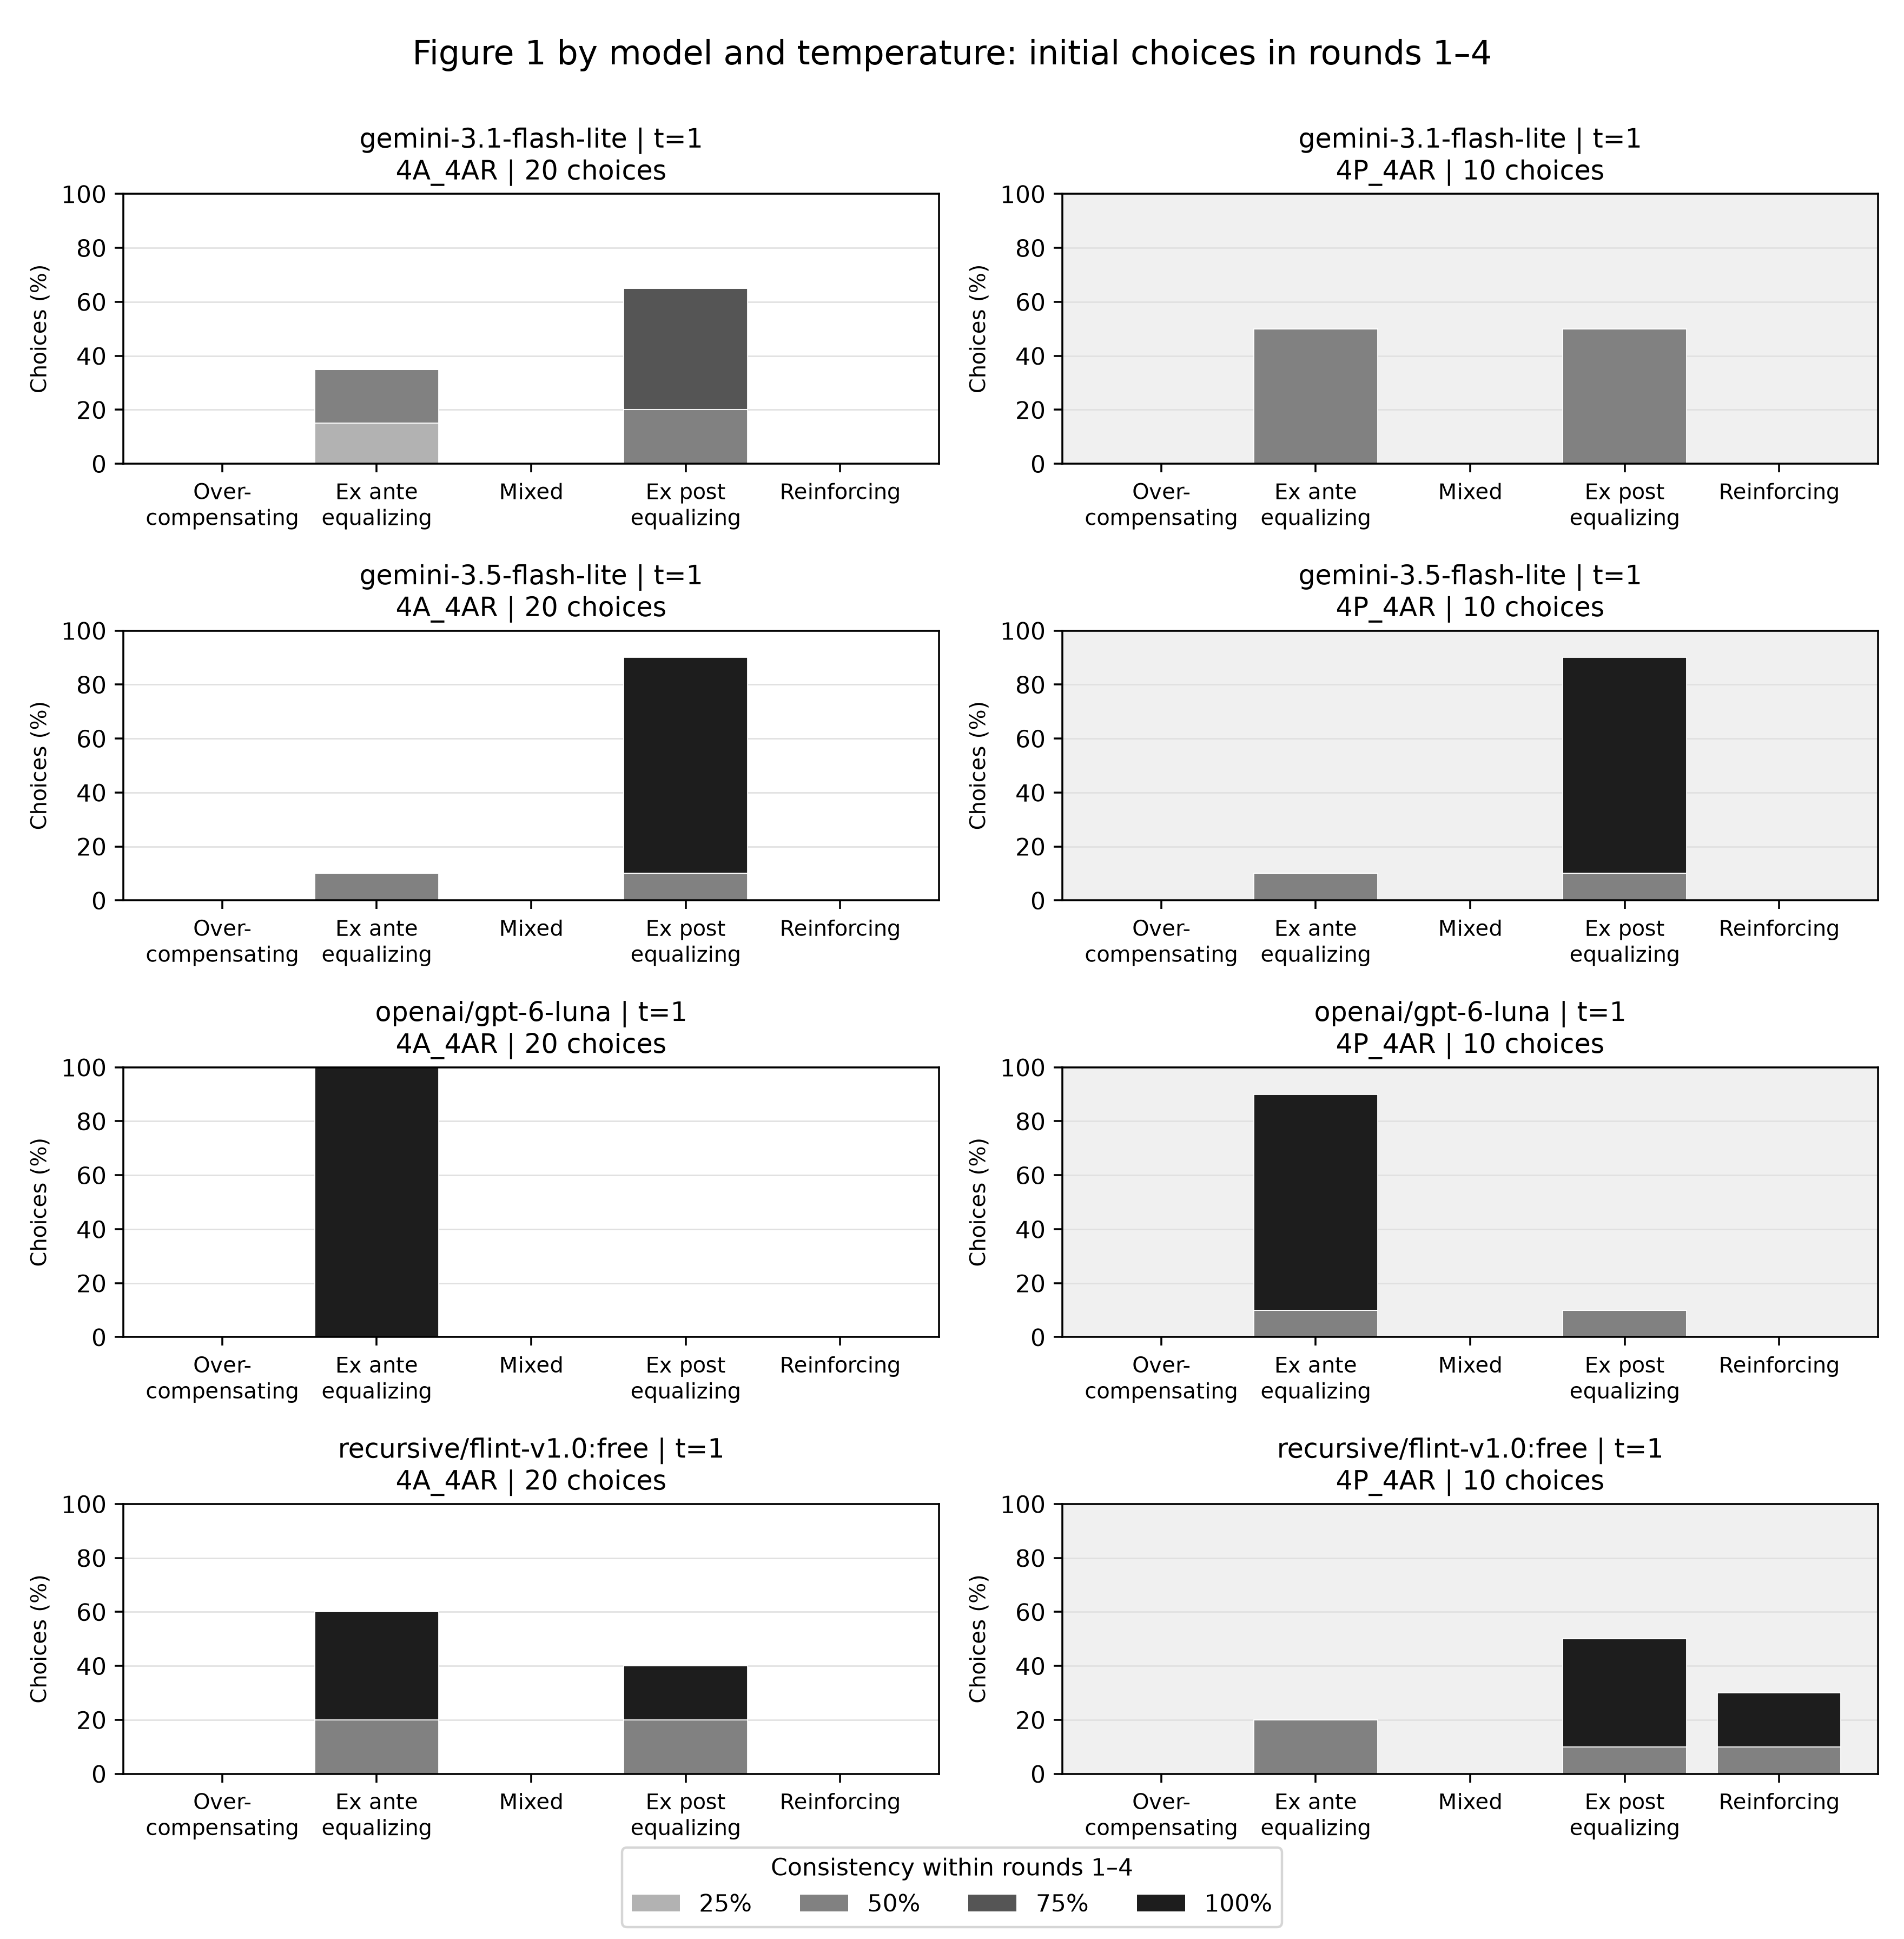
\includegraphics[width=\linewidth,height=.80\textheight,keepaspectratio]{04_fig1_by_model.png}
  \caption{Initial allocations in A and P tasks by model.}
  \label{fig:initial-choices-by-model}
\end{figure}

\clearpage
\begin{figure}[!htbp]
  \centering
  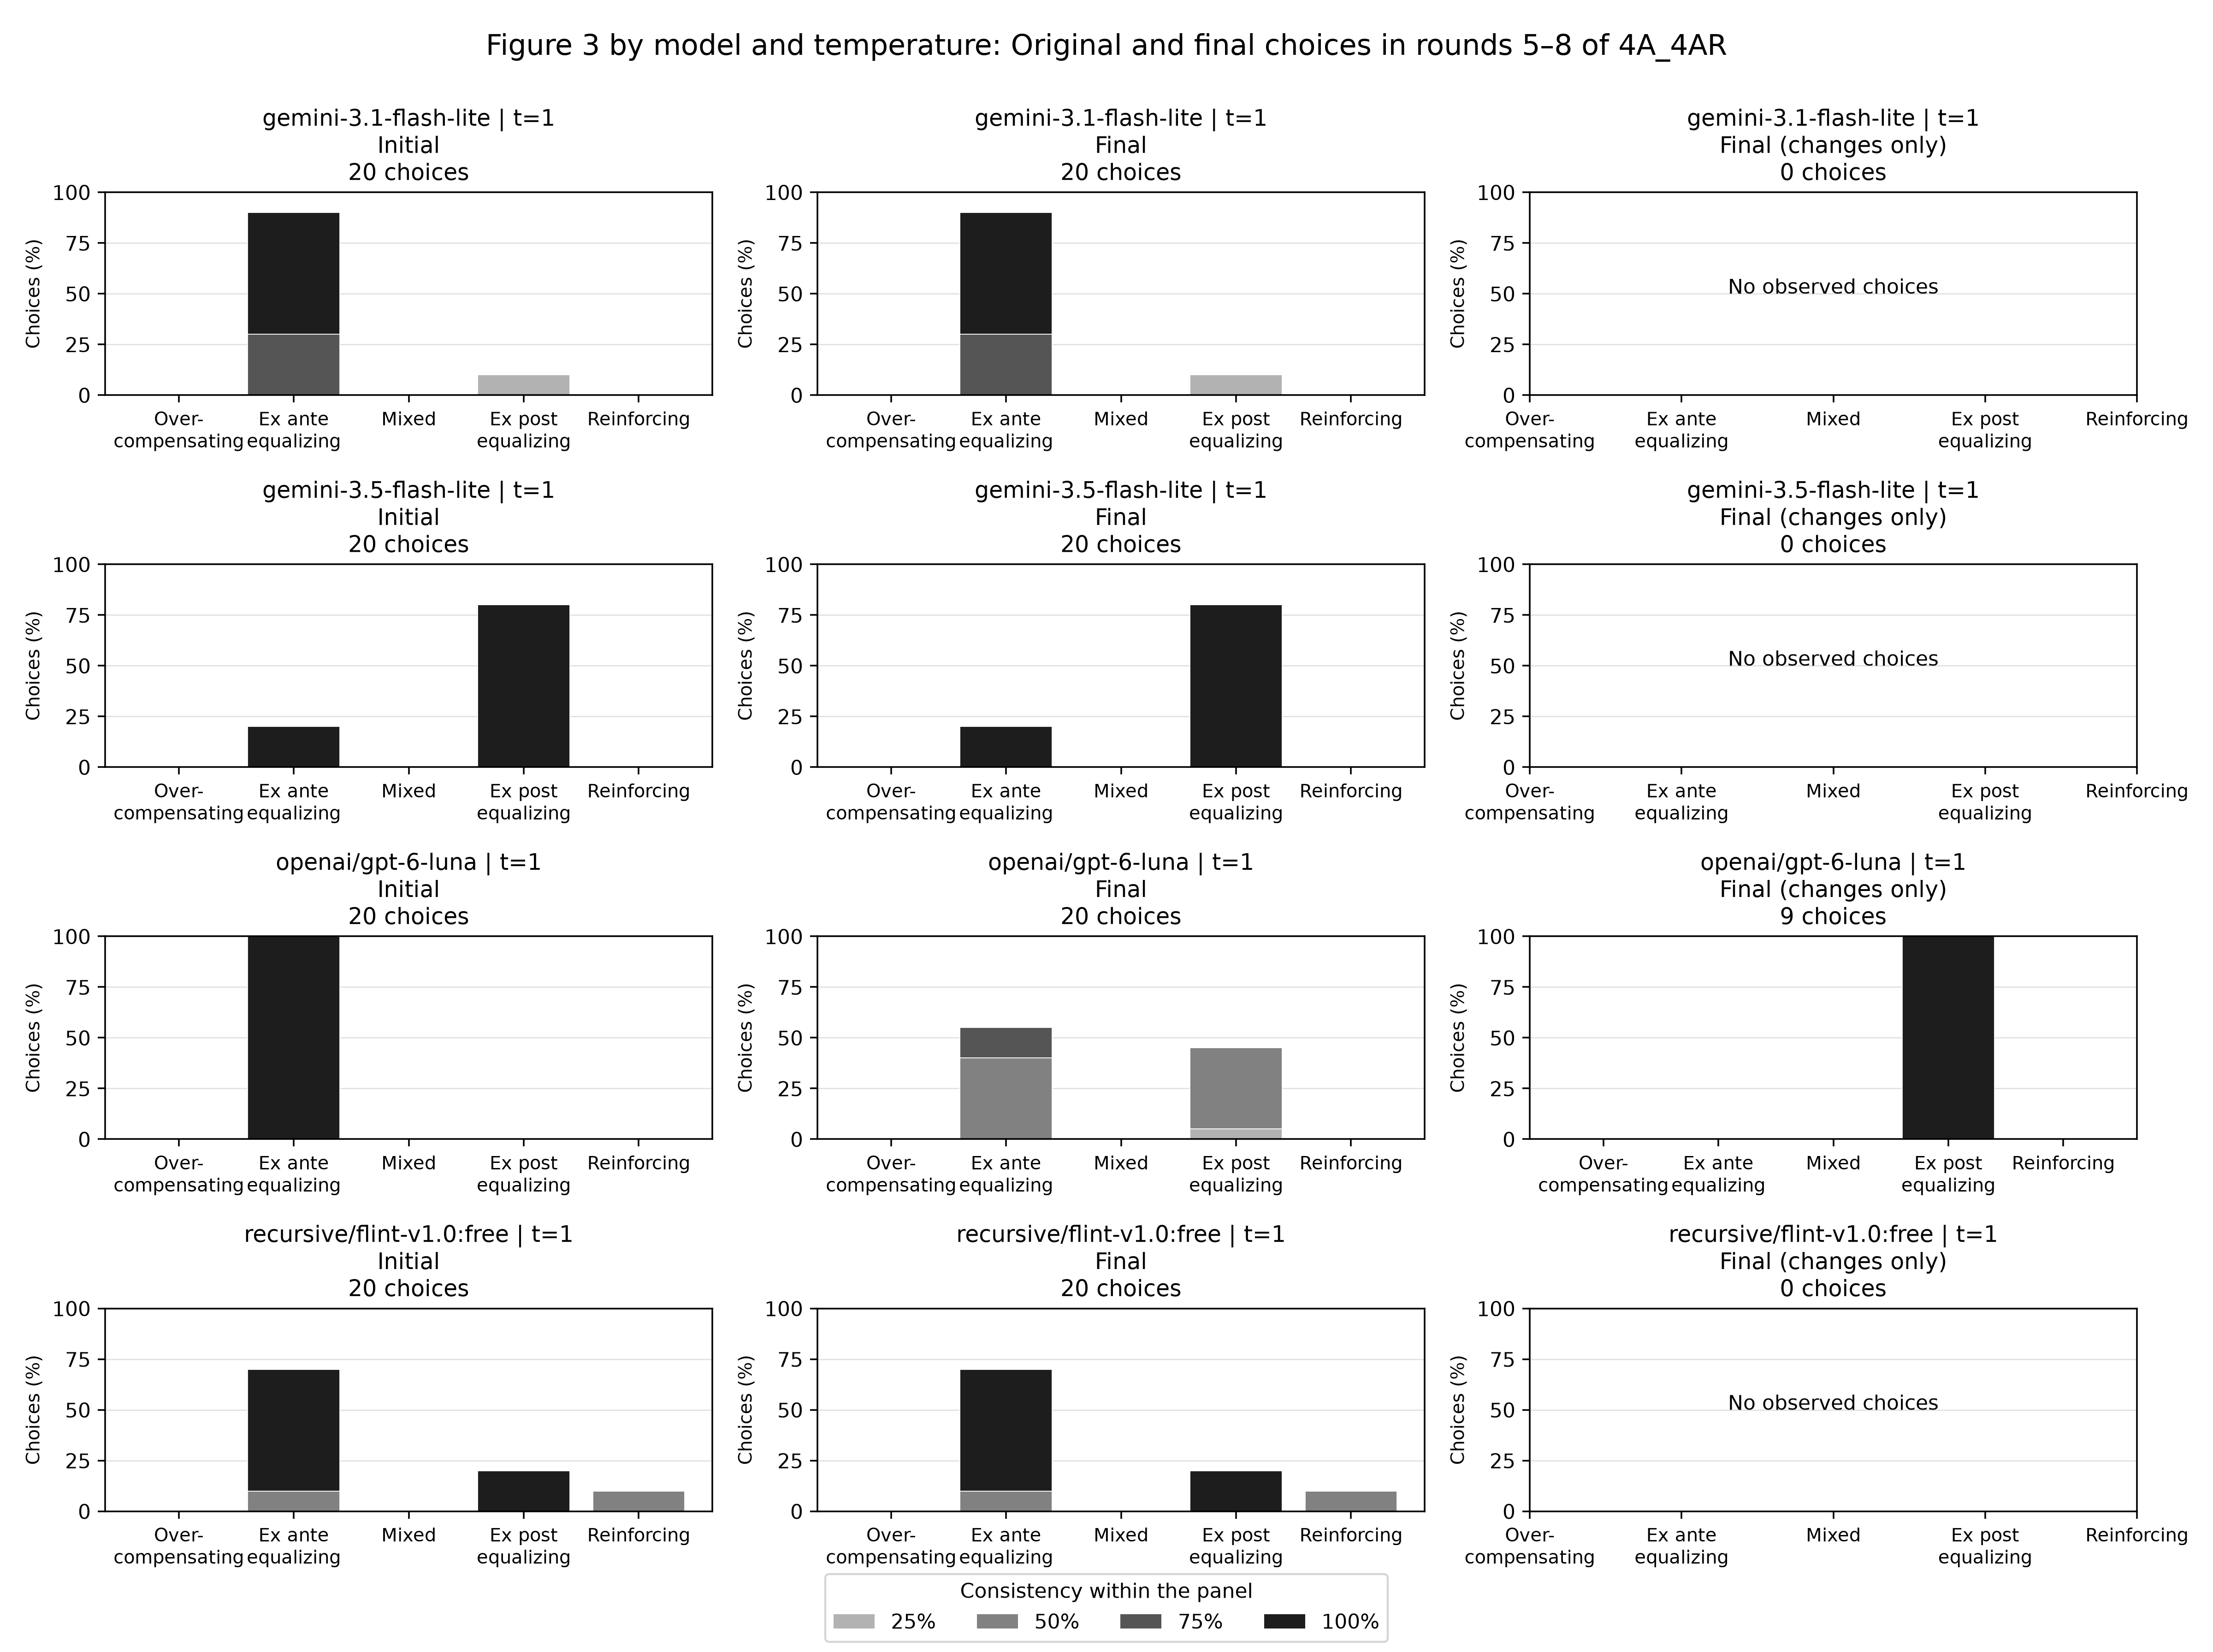
\includegraphics[width=\linewidth,height=.85\textheight,keepaspectratio]{05_fig3_by_model.png}
  \caption{Initial and final allocations in 4A\_4AR by model, rounds 5--8.}
  \label{fig:revisions-by-model}
\end{figure}

\clearpage
\section{Pilot prompt}
\label{app:prompts}
\begingroup
\singlespacing
\lstset{basicstyle=\fontsize{8.5}{9.5}\selectfont\ttfamily,columns=fullflexible,
        breaklines=true,breakatwhitespace=true,breakindent=1em,showstringspaces=false,keepspaces=true,upquote=true}
\IfFileExists{assets/pilot-prompts.txt}
  {\lstinputlisting{assets/pilot-prompts.txt}}
  {\lstinputlisting{../assets/pilot-prompts.txt}}
\endgroup
\clearpage
\section{Selected pilot prompts and responses}
\label{app:responses}
\begingroup\raggedright
These four \texttt{4A\_4AR} examples show exact prompt excerpts and complete raw replies. All allocation prompts ask for ten tickets split into integer A/B counts in one JSON object. Full questions and zero-based source indices are in \path{docs/assets/pilot-response-examples.txt}, checked by \path{analysis/check_pilot_replies.py}.\par
\endgroup

\begingroup
\singlespacing
\lstset{basicstyle=\fontsize{9}{10.2}\selectfont\ttfamily,columns=fullflexible,
        breaklines=true,breakatwhitespace=true,breakindent=1em,showstringspaces=false,keepspaces=true,upquote=true,
        aboveskip=3pt,belowskip=3pt}
\IfFileExists{assets/pilot-response-examples.txt}
  {\def\examplefile{assets/pilot-response-examples.txt}}
  {\def\examplefile{../assets/pilot-response-examples.txt}}

\noindent\textbf{1. Initial allocation.} GPT-6 Luna, player 3, round 5. JSONL line 61, messages 14--15.
\lstinputlisting[firstline=11,lastline=11]{\examplefile}
\lstinputlisting[firstline=17,lastline=18]{\examplefile}
This 2/8 allocation offsets the computer's 8/2, giving both households ten tickets overall.

\noindent\textbf{2. Revision after the reveal.} Same player and round. JSONL line 61, messages 23--24.
\lstinputlisting[firstline=30,lastline=32]{\examplefile}
\lstinputlisting[firstline=36,lastline=37]{\examplefile}
The player changes to 5/5 after learning that a participant ticket wins, a choice reversal.

\noindent\textbf{3. Code fences.} Gemini 3.5 Flash-Lite, player 0, round 1. JSONL line 21, messages 2--3.
\lstinputlisting[firstline=49,lastline=49]{\examplefile}
\lstinputlisting[firstline=55,lastline=58]{\examplefile}
The allocation is valid, but Markdown fences violate the requested single-object format.

\noindent\textbf{4. Repeated object.} Recursive Flint, player 0, round 3. JSONL line 1, messages 8--9.
\lstinputlisting[firstline=70,lastline=70]{\examplefile}
\lstinputlisting[firstline=76,lastline=77]{\examplefile}
The identical repeated object is a format deviation; the parser extracts the last valid allocation.
\endgroup
\end{document}
